\section{Computational Efficiency of Adaptive Multi-Fidelity BPSO}
\label{sec:amf-efficiency}
\subsection{Diagnosis and experimental correction}
The earlier matched-wall study gave each method 30 seconds with high iteration ceilings and no target-stop rule. It therefore measured quality at a common budget, not saving to a common quality: BPSO and UA each consumed about 28.76 GPU seconds. Predictor calls cost about 0.10 seconds; its archive cost 403.82 GPU seconds. Continuation and decoded deduplication already worked. Per-example batching, scalar synchronization, dense validation and repeated model/checkpoint loading were execution overheads.

We distinguish fixed-quality and fixed-compute experiments. For target $\tau$, define $T(\tau)$ as cumulative measured GPU elapsed when an actually evaluated 30-epoch candidate first reaches validation macro-F1 $\tau$. Misses are right-censored at budget $B$; restricted completion time is $\min(T,B)$. Every seed remains in the comparison. Fixed-compute experiments compare best actual 30-epoch scores at common GPU limits and cannot themselves prove cost saving.

GPU elapsed retains the original convention: synchronized training/validation elapsed time, including host stalls within those intervals; it is not pure kernel time or energy. Predictor, scheduling, checkpoint and import overhead also appears in search wall time. GPU caps are checked at completed epoch boundaries, so a last epoch can overrun. Strict-budget score comparisons exclude terminal observations after the stated limit.

\subsection{Engineering and candidate policy}
Vectorized batches preserve the original sampler and RNG order. Bounded data/resident-tensor caches reduce loading/transfers, and a one-model cache keyed by trial directory avoids redundant reconstruction and optimizer loading during immediate continuation. FP32 loss-scalar synchronization is deferred. Validation runs at 3/10/30 epochs; checkpoints still commit each epoch. Across three development architectures, cumulative GPU elapsed fell from 25.059 to 20.182 seconds (19.47\%), with identical final parameter tensors. Fixed-order one-pass profiles have limited precision. AMP changed outcomes beyond the 0.01 development tolerance and was rejected; batch sizes/search space were unchanged.

The candidate initially probes two particles, then chooses continuations dynamically rather than using a fixed halving quota. A new probe is forced after at most two promotions. Its priority is
\begin{equation}
\begin{split}
P(a)={}&\widehat f_{30}(a)+\beta u(a)\\
&-\lambda\frac{\widehat c(a)}{\operatorname{median}_{z\in\mathcal A}\widehat c(z)}.
\end{split}
\end{equation}
where $\widehat c$ separates remaining training epochs from remaining validation passes. A candidate is stopped if its full prediction upper bound is below the best observed 30-epoch score plus 0.01; low initial F1 alone does not stop it. Only actual terminal scores update BPSO attractors. All predictive variants retain the same 20\% diversity restart.

The sparse, timing-invariant forest is refit using existing logs. Architecture-disjoint development replay on IDs 0--11 fixed $\beta=0.1$, $\lambda=0.2$ before the new search seeds. Calibration IDs 12--17 and held-out IDs 18--24 retain the split-conformal residual construction~\cite{angelopoulos2021}. Nominal 80\% intervals covered 13/14 held-out observations at 3 epochs and 14/14 at 10, with mean widths 0.573 and 0.481. These broad intervals do not guarantee useful calibration under adaptive proposal shift. No new GPU archive was collected; historical collection cost is still charged.

\subsection{Measured quality, cost and ablations}
Nine methods/ablations used seeds 601--603, the same 8192/4096 training/validation view, all eight classes, original training-fitted Min--Max preprocessing, balanced loss, FP32 runtime and maximum fidelity 30. The initial 8-GPU-second pilot executed independent targets 0.4/0.5/0.6 and fixed-compute runs. Low control attainment motivated a declared exploratory continuation to 20 GPU seconds for target 0.6 and fixed compute. It retained all methods/seeds/coefficients, resumed saved optimizer/RNG states, and charged every previously spent epoch, GPU second and wall second, including checkpoint-import overhead. It is not a new independent replication.

\begin{table}[!t]\centering\caption{Target 0.6: actual mean GPU elapsed to target or cap, with all three seeds retained. Misses are censored rather than excluded. Scores are actual terminal validation macro-F1. Archive cost is separate.}\label{tab:amf-compute}
\resizebox{\columnwidth}{!}{\begin{tabular}{lrrrr}\toprule
Method & GPU s & F1 & Saving (\%) & Hits\\\midrule
BPSO & 17.01 & 0.264 & 0.0 & 1/3\\
BPSO-SH & 12.10 & 0.497 & 28.8 & 2/3\\
DEHB & 6.78 & 0.703 & 60.2 & 3/3\\
Fixed prediction & 11.94 & 0.529 & 29.8 & 2/3\\
Hyperband & 17.88 & 0.502 & -5.1 & 1/3\\
Dynamic prediction & 12.98 & 0.507 & 23.7 & 2/3\\
Full UA & 12.80 & 0.539 & 24.7 & 2/3\\
UA without cost & 13.03 & 0.507 & 23.4 & 2/3\\
UA without bonus & 12.80 & 0.539 & 24.7 & 2/3\\
\bottomrule\end{tabular}
}
\end{table}
Full UA used 12.803 GPU seconds versus 17.008 for BPSO: a 24.72\% online reduction, just below the 25\% engineering goal. It attained 2/3 targets versus 1/3 for BPSO. SH used 12.103 seconds with 2/3 hits, so full UA was 5.78\% slower. DEHB used 6.776 seconds, attained 3/3 targets and saved 60.16\% versus BPSO. These finite-horizon, three-seed results do not establish statistical superiority. The restricted-time saving 25.14\% is a different censored estimand and must not replace the actual-consumption result to claim the 25\% goal was met.

\begin{figure}[!t]\centering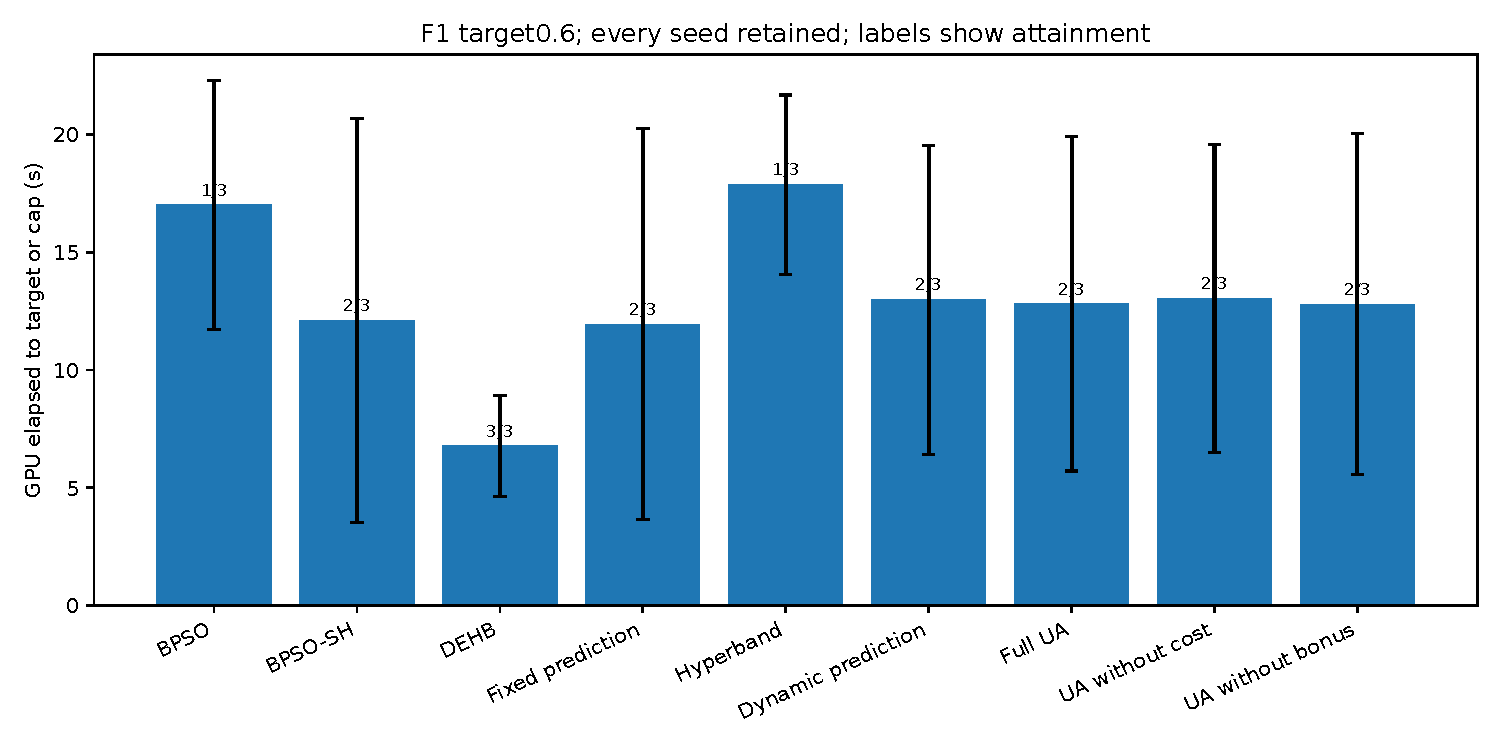
\includegraphics[width=\columnwidth]{../../results/ua_amf_efficiency_20261108/target_cost.pdf}
\caption{Actual target-or-cap GPU consumption, including misses. Error bars show search-seed SD; annotations give target attainment.}\end{figure}
\begin{figure}[!t]\centering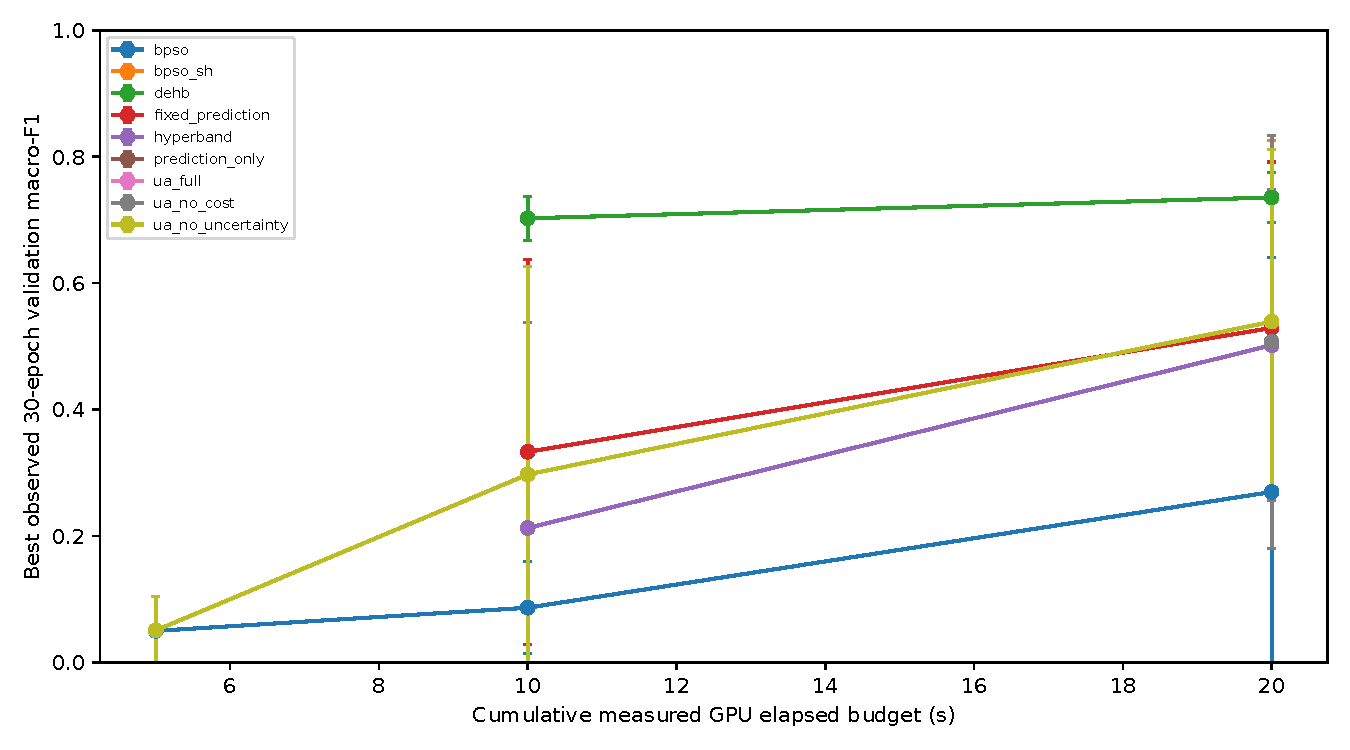
\includegraphics[width=\columnwidth]{../../results/ua_amf_efficiency_20261108/followup20/gpu_anytime.pdf}
\caption{Fixed-compute quality at 5/10/20 GPU seconds. Means/SD require all three seeds to have a terminal model; missing points are not replaced by zero. Raw seed traces are also retained.}\end{figure}
At fixed 20-second compute, mean validation macro-F1 was 0.5391 for full UA,0.2696 for BPSO,0.5030 for SH and 0.7356 for DEHB. The full-method gap to DEHB was 0.1965, exceeding the 0.02 preservation margin. Removing the uncertainty bonus changed no terminal winner scores. Removing cost reduced mean F1 by 0.0320, but cost-aware UA still did not beat SH on target-time cost. Fixed-quota prediction used 11.940 target-or-cap GPU seconds and F1~0.5291; dynamic prediction used 12.978 and 0.5071. The more complex allocation is not independently supported as an improvement.

\subsection{Total cost, final models and limitations}
Charging the historical archive gives 416.622 GPU seconds for one full-UA quality search versus 17.008 for BPSO: no net single-search saving remains. The fit/calibration subset alone cost 308.386 historical GPU seconds. Smaller-log CPU refits reduced that attributable subset but increased held-out point-prediction error; they were not substituted into the frozen benchmark. Historical reuse is not free computation. Online calibration was not claimed from a few adaptively selected terminal observations.

All methods' fixed-compute architecture choices were frozen before final testing, using dedicated seed 1601 and 30 epochs. The previously examined historical test is not blind independent data. BPSO test macro-F1 was 0.2733, with normal FPR 0.8038. BPSO-SH test macro-F1 was 0.5759, with normal FPR 0.6180. Full UA test macro-F1 was 0.3100, with normal FPR 0.9442. DEHB test macro-F1 was 0.6859, with normal FPR 0.7549. Precision, attack recalls, confusion matrices, parameters and measured inference latency are retained; one final training seed and shared historical rows limit generalization. Existing conventional MLP/CNN/GRU/reference results remain contextual.

At the preceding study stage, the regression suite passed 105 CPU and 50 targeted CUDA tests. Saved validation/test predictions were re-scored, epoch ledgers were checked, and the old manuscript and results were preserved.

The strongest measured free control is DEHB; SH is the simpler BPSO alternative and beats full UA on target-time cost. Runtime engineering is verified, but novelty and superior uncertainty-aware allocation are not established. The initial pilot and exploratory extension are reported separately; more search/final seeds, full-training studies, independently validated calibration and independent captures remain necessary.

\subsection{Archive-free online extension}
The archive-dependent result above motivated a fresh, separately bounded experiment. The new implementation starts with precisely ordinary BPSO--SH proposals, quotas and tie handling. It captures architecture, learning-curve prefix and measured incremental-cost features at epochs 3 and 10, attaching a terminal label only after actual epoch 30 training. No offline bundle, historical target, cross-method checkpoint or separately trained GPU archive enters this variant. Candidate maturation is charged to ordinary search work.

A fixed architecture hash assigns fit/calibration/check roles with expected proportions 50/20/30\%. CPU random forests use 24 trees of maximum depth 4. All current query architectures are excluded from fitting and calibration. Check forecasts are frozen before their terminal labels arrive. At least six fit, four calibration and four prequential check architectures per rung are required. The point gate requires MAE$\leq0.08$, at least 10\% and 0.005 absolute MAE improvement over current-F1 prediction, and Spearman$\geq0.3$. For uncertainty modes, empirical coverage must be at least 0.75 for nominal 80\% intervals, with mean width at most 0.3; current intervals must also meet the width limit. These are conservative engineering checks, not a proof of calibration under adaptive sampling.

The interval uses a separate calibration quantile of absolute residual divided by forest dispersion (floor 0.02). If useful, ranking uses the earlier priority equation with generic frozen $\beta=0.1$, $\lambda=0.05$ and median-normalized measured remaining cost. Prediction-only sets both coefficients to zero; uncertainty-only sets $\lambda=0$. Failure of a gate retains ordinary SH ranking. Only actual terminal observations update swarm bests. Fixed SH quotas are intentionally retained to isolate ranking; no new BPSO equation or algorithmic novelty is claimed.

\subsection{Fresh end-to-end comparison}
The 42 new runs use seeds 601--603, seven methods, target 0.6 and fixed 20-GPU-second phases. Dataset rows, eight labels, preprocessing, architecture space, FP32 execution and 3/10/30 fidelities match the preceding 20-second experiment. A 50-second wall safety cap also applies. Method order is a seeded permutation; methods run serially. Earlier checkpoints are not imported. Misses are retained and censored; strict-horizon quality excludes terminal evaluations beyond the cap, while actual resource consumption includes epoch-boundary overruns. Times follow the existing synchronized elapsed convention.

\begin{table}[!t]\centering\caption{Fresh target 0.6 runs, means across three search seeds. GPU seconds are measured; archive cost is charged to a standalone search. All misses are retained. Hits count actual terminal targets before the strict horizon.}\label{tab:online-quality}
\resizebox{\columnwidth}{!}{\begin{tabular}{lrrrrr}\toprule
Method & Online GPU & Archive & Total GPU & F1 & Hits\\\midrule
BPSO & 16.824 & 0.00 & 16.824 & 0.3054 & 1/3\\
BPSO + SH & 12.004 & 0.00 & 12.004 & 0.4971 & 2/3\\
DEHB & 6.778 & 0.00 & 6.778 & 0.7026 & 3/3\\
Offline UA & 12.631 & 403.82 & 416.450 & 0.5391 & 2/3\\
Online prediction & 11.919 & 0.00 & 11.919 & 0.4971 & 2/3\\
Online + uncertainty & 11.950 & 0.00 & 11.950 & 0.4971 & 2/3\\
Archive-free full & 11.947 & 0.00 & 11.947 & 0.4971 & 2/3\\
\bottomrule\end{tabular}
}\end{table}

Archive-free full consumed 11.947 GPU seconds versus 16.824 for BPSO, a 28.99\% total reduction, with 2/3 versus 1/3 target attainment. Terminal validation macro-F1 means were 0.4971 and 0.3054 respectively. SH consumed 12.004 seconds and produced identical winner scores to the archive-free variants. The small 0.47\% timing difference does not establish an advantage over SH. DEHB used 6.778 seconds and reached 3/3 targets. Removing the archive lowers standalone total cost relative to offline UA (416.450 seconds), but the online component itself must earn its cost.

Across the 18 matched online trials, predictive promotion activated 0 times and CPU fitting ran 0 times. Thus the new modes effectively executed SH in this short-budget study. Their ablations do not establish any benefit from uncertainty or cost ranking. The zero external archive cost is real; an online-learning advantage is not demonstrated. CPU preparation ranged 0.0017--0.0078 seconds per run and is included in search wall time.

At fixed 20-second compute, archive-free full preserved SH scores but trailed offline UA by 0.0361 and DEHB by 0.2325 absolute macro-F1. Both exceed the 0.02 engineering preservation margin; competitive quality against the strongest control was not maintained.

\begin{table}[!t]\centering\caption{Fresh fixed 20-GPU-second comparison. F1 is best genuinely evaluated 30-epoch validation macro-F1, mean (sample SD). Epoch counts and actual GPU elapsed include charged incremental work.}\label{tab:online-compute}
\resizebox{\columnwidth}{!}{\begin{tabular}{lrrr}\toprule
Method & Terminal F1 (SD) & Epochs & GPU s\\\midrule
BPSO & 0.2696 (0.3715) & 178.7 & 20.040\\
BPSO + SH & 0.5030 (0.3231) & 138.3 & 20.088\\
DEHB & 0.7356 (0.0402) & 195.0 & 20.044\\
Offline UA & 0.5391 (0.2719) & 205.0 & 20.201\\
Online prediction & 0.5030 (0.3231) & 137.3 & 20.086\\
Online + uncertainty & 0.5030 (0.3231) & 137.3 & 20.089\\
Archive-free full & 0.5030 (0.3231) & 137.7 & 20.080\\
\bottomrule\end{tabular}
}\end{table}
\begin{figure}[!t]\centering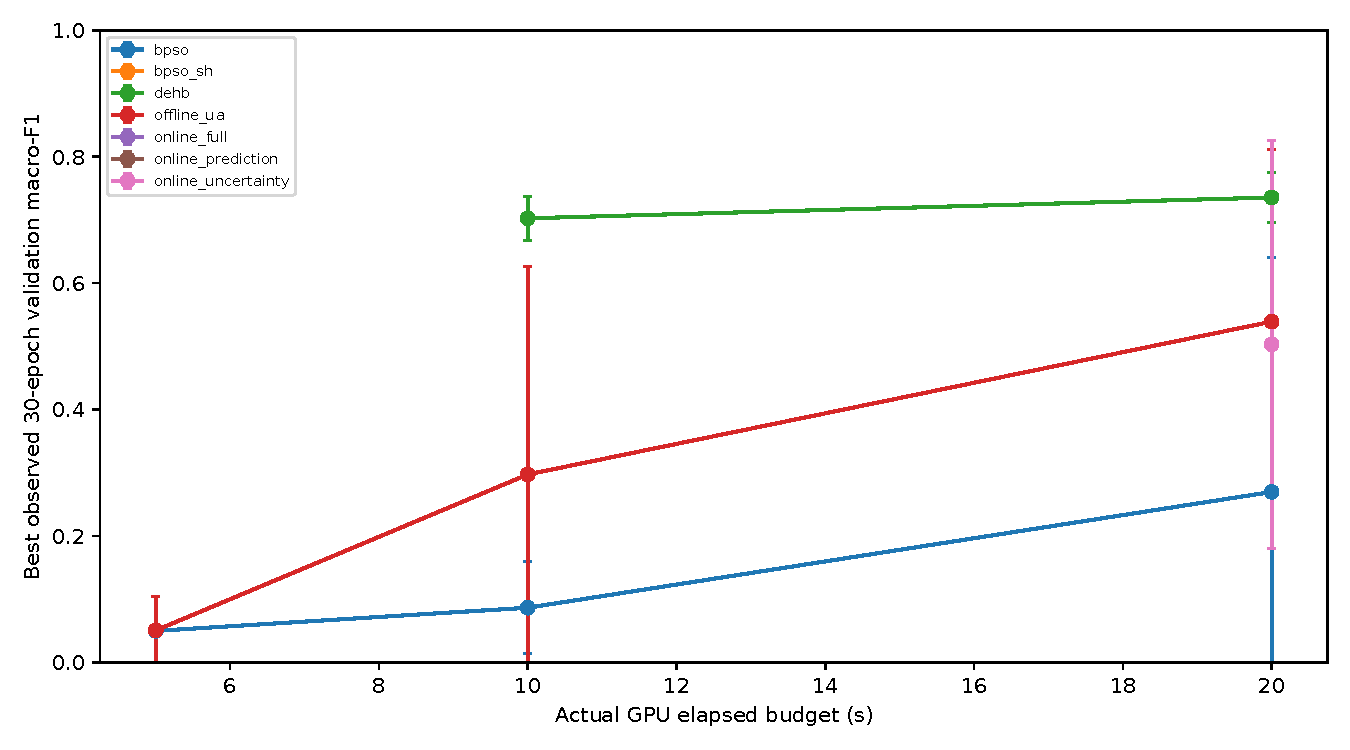
\includegraphics[width=\columnwidth]{../../results/ua_amf_online_20261108/anytime.pdf}
\caption{Fresh fixed-compute anytime quality. Error bars show search-seed SD; points require all three terminal scores. Equal budget consumption is not evidence of cost saving.}\end{figure}

The full archive is charged once for a reusable multi-search campaign in the accompanying CSV, rather than once per seed. Offline CPU development preparation is not fully isolated; recorded archive wall time 420.722 seconds therefore supplies only a lower bound for full offline wall preparation. Online CPU fitting/inference and scheduler costs are recorded separately. All saved validation predictions were independently re-scored, and epoch/GPU ledgers and architecture-disjoint feature/predictor identities were verified. The expanded suite passed 110 CPU and 55 targeted CUDA-configured tests.

The separate seed 601 diagnostic used 120.061 GPU seconds and 128.449 wall seconds, matured 16 distinct terminal architectures, performed 1 CPU fits and applied prediction at 0 promotion decisions. Preparation consumed 0.0475 CPU wall seconds. Gate counts: insufficient fit or calibration architectures: 32; insufficient out of time check architectures: 1. This is a cold-start diagnostic, not a matched performance comparison.

No new final detector test was executed in this extension. The preceding historical test results are retained, and the test remains development-known. The evidence supports removing an uneconomic archive and using SH fallback; it does not support superior online uncertainty-aware allocation. DEHB remains the strongest measured control, with SH the simpler BPSO alternative. More seeds, a prespecified larger matched horizon, useful online calibration and independent data remain necessary before an IEEE optimizer contribution can be defended.
